\documentclass[
	classe=$1^{ere}STI2D$,
	landscape,
	twocolumn,
	headerTitle={Interrogation}
]{évaluation}

\setlength{\columnsep}{1cm}
\renewcommand{\arraystretch}{1.3}

\date{9 décembre 2022}

\begin{document}

%%%%%%%%%%%%%%%%%%%%%%%%%%%%%%%%%%%%%%%%%%%%%%%%%
% SUJET A
%%%%%%%%%%%%%%%%%%%%%%%%%%%%%%%%%%%%%%%%%%%%%%%%%

\title{Interrogation : fonctions du 2ⁿᵈ degré (sujet A)}
\maketitle

On donne les fonctions $A(x) = x² + 2x + 3$ et $B(x) = -\frac{1}{2}x² + 3x + 4$.


\begin{enumerate}
	\item Donner l'expression de

	      $$ f(x) = A(x) - B(x) = \correctionDots{\frac{1}{2}x² - x - \frac{3}{2}} $$
	\item Placer dans le repère ci-dessous les points

	      $(-2 ; f(-2))$, $(-1 ; f(-1))$, $(0 ; f(0))$, $(1 ; f(1))$ et $(2 ; f(2))$
	      \newcommand{\fonctionF}[1]{%
		      0.5*#1*#1 - #1 - 1.5%
	      }
	      \begin{center}
		      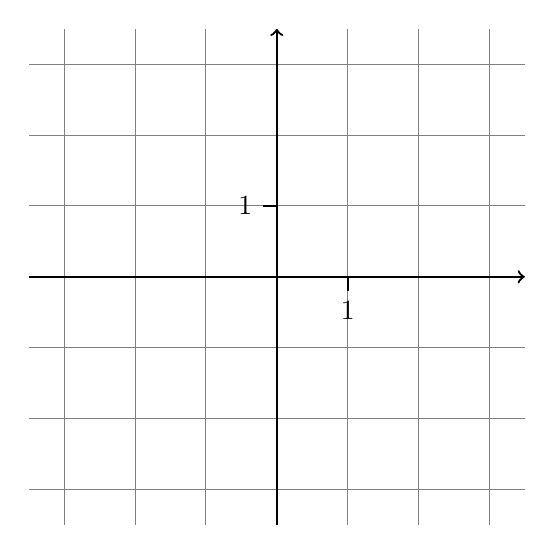
\begin{tikzpicture}[scale=0.9]
			      \draw[thin,gray] (-3.5,-3.5) grid (3.5,3.5);
			      \draw[thick,->] (-3.5,0) -- (3.5,0);
			      \draw[thick,->] (0,-3.5) -- (0,3.5);
			      \draw[thick] (1,0) -- ++(0,-0.2) node[below] {$1$}
			      (0,1) -- ++(-0.2,0) node[left] {$1$};
			      \ifdefined\makeCorrection
				      \foreach \x in {-2,...,2} {
						      \node[red] at (\x,\fonctionF{\x}) {×};
					      }
			      \fi
		      \end{tikzpicture}
	      \end{center}
	\item Montrer que $f(x)$ peut s'écrire $\frac{1}{2}(x - 3)(x + 1)$ :

	      \ifdefined\makeCorrection
		      \color{red}
		      \begin{align*}
			      \frac{1}{2}(x - 3)(x + 1) & = \frac{1}{2}(x² - 3x + x - 3)    \\
			                                & = \frac{1}{2}(x² - 2x - 3)        \\
			                                & = \frac{1}{2}x² - x - \frac{3}{2} \\
			                                & = f(x)                            \\
		      \end{align*}
	      \fi
\end{enumerate}

\newpage
\setcounter{exercice}{1}
%%%%%%%%%%%%%%%%%%%%%%%%%%%%%%%%%%%%%%%%%%%%%%%%%
% SUJET B
%%%%%%%%%%%%%%%%%%%%%%%%%%%%%%%%%%%%%%%%%%%%%%%%%

\title{Interrogation : fonctions du 2ⁿᵈ degré (sujet B)}
\maketitle

On donne les fonctions $A(x) = x² + 3x + 3$ et $B(x) = -\frac{1}{2}x² + 2x + 4$.


\begin{enumerate}
	\item Donner l'expression de

	      $$ f(x) = A(x) - B(x) = \correctionDots{\frac{1}{2}x² + x - \frac{3}{2}} $$
	\item Placer dans le repère ci-dessous les points

	      $(-2 ; f(-2))$, $(-1 ; f(-1))$, $(0 ; f(0))$, $(1 ; f(1))$ et $(2 ; f(2))$
	      \newcommand{\fonctionF}[1]{%
		      0.5*#1*#1 + #1 - 1.5%
	      }
	      \begin{center}
		      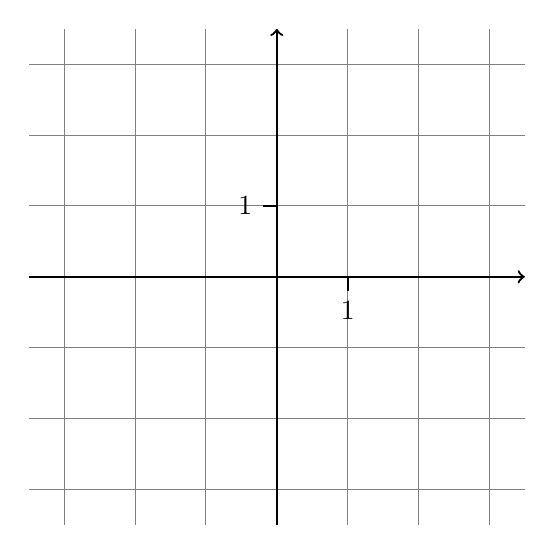
\begin{tikzpicture}[scale=0.9]
			      \draw[thin,gray] (-3.5,-3.5) grid (3.5,3.5);
			      \draw[thick,->] (-3.5,0) -- (3.5,0);
			      \draw[thick,->] (0,-3.5) -- (0,3.5);
			      \draw[thick] (1,0) -- ++(0,-0.2) node[below] {$1$}
			      (0,1) -- ++(-0.2,0) node[left] {$1$};
			      \ifdefined\makeCorrection
				      \foreach \x in {-2,...,2} {
						      \node[red] at (\x,\fonctionF{\x}) {×};
					      }
			      \fi
		      \end{tikzpicture}
	      \end{center}
	\item Montrer que $f(x)$ peut s'écrire $\frac{1}{2}(x - 1)(x + 3)$ :

	      \ifdefined\makeCorrection
		      \color{red}
		      \begin{align*}
			      \frac{1}{2}(x - 1)(x + 3) & = \frac{1}{2}(x² - x + 3x - 3)    \\
			                                & = \frac{1}{2}(x² + 2x - 3)        \\
			                                & = \frac{1}{2}x² + x - \frac{3}{2} \\
			                                & = f(x)                            \\
		      \end{align*}
	      \fi
\end{enumerate}

\end{document}